\documentclass[final,11pt]{article}
\usepackage{times}
\usepackage{epsfig}
\usepackage{multirow} 
\usepackage[left=.80in,top=.85in,right=.80in,bottom=.85in]{geometry}
% 14.5 pages:
% \usepackage[left=.78in,top=.74in,right=.78in,bottom=.75in]{geometry}
% lots of margin:
% \usepackage[left=1.00in,top=1.00in,right=1.00in,bottom=1.00in]{geometry}
%\usepackage{subfigure}
\usepackage{subcaption}
\usepackage{enumerate}
\usepackage{afterpage}
\usepackage{sectsty}
\usepackage{enumitem}
\usepackage{colortbl} 
\usepackage{graphicx}
\usepackage{setspace}
\usepackage{bibspacing}
\usepackage{url}
\usepackage{gensymb}
\usepackage{pgfgantt}
\newif\ifcmm
\cmmfalse
\long\def\CMM#1{
\ifcmm #1\else\relax\fi}
\def\thechapter{./}
\usepackage{moreepsf}
\long\def\AuthorNote#1{%
{\Large\bf #1}}
\def\Action#1{\texttt{#1}}
\def\TiC{{\sc corc}}

\definecolor{purple}{rgb}{.6,.2,.4} 
\definecolor{ltblue}{rgb}{.6,.6,1}

\newcommand{\ignore}[1]{ }
\graphicspath{{./}{figures/}}
%for comments
\newcommand{\FIXME}[1]{\textcolor{red}{FIXME: #1}}

% Shrink space in enums and lists
\setlist{topsep=3pt,itemsep=3pt,parsep=3pt}
\setlist[1]{labelindent=\parindent}

% Bolded figure captions in the ACM style
\makeatletter
\long\def\@makecaption#1#2{%
   \vskip 10\p@
   \setbox\@tempboxa\hbox{{\bf#1: #2}}%
   \ifdim \wd\@tempboxa >\hsize
    {\bf #1: #2}\par
     \else
       \hbox to\hsize{\hfil\box\@tempboxa\hfil}%
   \fi}
\makeatother


% Make bullet list singled spaced
\newenvironment{packed_item}{
\begin{list}{\labelitemi}{%
  \leftmargin=1.0em
  \setlength{\itemsep}{3pt}
  \setlength{\parskip}{0pt}
  \setlength{\parsep}{3pt}
}
}{\end{list}}

\def\paragraph#1{%

\smallskip

\noindent{\bf #1}\hbox to 1em{\hss}%
}

\newenvironment{rquote}{\setlength{\leftmargini}{1em}\setlength{\leftmarginii}{1em}\quotation\noindent}{\endquotation}

% Make enumberated list singled spaced
\newenvironment{packed_enum}{
\begin{enumerate}
  \setlength{\itemsep}{1pt}
  \setlength{\parskip}{0pt}
  \setlength{\parsep}{0pt}
}{\end{enumerate}}



% Modify the default section and subsection headers
\makeatletter
\def\@seccntformat#1{\@ifundefined{#1@cntformat}
{\csname the#1\endcsname\,}
{\csname #1@cntformat\endcsname}
}
\def\section@cntformat{\thesection.\,}
\def\subsection@cntformat{\thesubsection.\,}
\def\subsubsection@cntformat{\thesubsubsection.\,}

%phjones changed to 1, 2, 2.1 ...
%\def\thesection{\Roman{section}}
%\def\thesubsection{\thesection.\Alph{subsection}}
%\def\thesubsubsection{\thesubsection.\arabic{subsubsection}}
%\makeatother

%phjones changed to 1, 2, 2.1 ...
\def\thesection{\arabic{section}}
\def\thesubsection{\thesection.\arabic{subsection}}
\def\thesubsubsection{\thesubsection.\arabic{subsubsection}}
\makeatother

\sectionfont{\normalsize\MakeUppercase}
\subsectionfont{\normalsize}


% Create a non-indented bolded start to a paragraph.
\newcommand{\npara}[1]{\noindent{\bf #1}}


% Increase the space between paragraphs.
\setlength{\parskip}{.8ex plus 0.5ex minus 0.2ex} 


%for comments
\newcommand{\alvitta}[1]{\textcolor{cyan}{Alvitta: #1}}

\pagestyle{empty}
\begin{document}
\thispagestyle{empty}
\setcounter{page}{0}

\begin{center}
{\Large
Practical Privacy in the Internet of Things
}

\vskip 0.2in
{\sc Todd Steinbrueck}
\\BECS Technology, Inc., St. Louis, Missouri
\vskip 0.05in
Email: todd@becs.com
\end{center}

\clearpage
\section*{Project Summary}

%Overview description (potential outcome(s) of the proposed activity
%in terms of a product, process, or service).
%
%--End of instructions--

Electronic control systems in the modern era are regularly connected
to the Internet, becoming endpoint nodes in the Internet-of-Things (IoT).
It is common for these control systems to log (over time) sensor measurements,
control decisions, anomalous or alarm conditions, parameter settings,
and the like; and these data can be helpful in verifying compliance to
relevant regulations, improving control function, diagnosing problems,
and maintaining appropriate stocks of consumables.

An individual organization, however, is limited to seeing only the data logs
of control systems that it directly owns. Aggregating data from multiple
systems (crossing organizational boundaries) can provide benefits to all
owners of similar equipment (e.g., better knowledge of the impact of
control decisions, diminished usage of consumables, prediction of future
problems). We propose to provide anonymized data sets for mining, utilizing
the strong guarantees made available by differential privacy techniques.

\paragraph{Key Words:} IoT, differential privacy

\paragraph{Subtopic Name:} IT4. Cybersecurity; Authentication; Privacy

\medskip

\paragraph{Intellectual Merit}
This Small Business Technology Transfer Research Phase I project will
investigate
the practical viability of providing differential privacy guarantees to
owners of data collected by IoT devices.  We will attempt to answer the
question, ``Can differential privacy theory be effectively reduced to
practice?'' for IoT data.

BECS Technology, Inc., (BECS) manufactures control equipment in a
number of markets.
This equipment is part of the Internet-of-Things, and BECS takes the
security and privacy of its equipment, and data collected from that
equipment, very seriously.
Our approach to data privacy has historically been one based strictly 
on ownership, the owner of the equipment is the owner of the data from
that equipment, and the owner is the only one who is allowed access to
that data.
This research will investigate the viability of relaxing that strict,
owner-based partitioning of the data.  More can be learned from aggregated
data sets, yet owners must be assured that by sharing their data the
benefits outweigh the risks.

In collaboration with Washington University in St.~Louis, we will develop an integrated system that aggregates clients' data to better harness the power of the IoT.  
In particular, this research agenda has two complementary veins. (1) 
Through empirical study,
we will assess the tradeoffs inherent in differentially private 
data science (i.e., what can be learned from the data, at what ``privacy
budget'').
This investigation will be carried out using aquatics data from
controllers manufactured by BECS and installed primarily in North America
(and extending around the world).
(2) We will explore visualization designs for displaying this aggregated data as well as methods for representing data uncertainty. 
We will conduct a series of empirical studies to compare existing techniques for representing time series data and uncertainty to non-experts. 
Together, the results of these two research trajectories will give us the means to combine data in a privacy-preserving manner and enable clients to better understand their data to support decision-making.  



\medskip

\paragraph{Commercial/Broader Impacts}
Providing practical and effective privacy guarantees for IoT-derived data
is potentially transformative, not only for the markets that BECS currently
serves, but across the entire range of devices in the IoT.
By encouraging the owners of data to be willing to share data while having
strong assurances their privacy will be preserved, more data will be
willingly shared, to the greater societal good.

Education -- This project will be carried out in collaboration with
Washington University in St. Louis, supporting two graduate students.
The students will be trained with an appropriate balance of expertise in human reasoning, state-of-the-art privacy theory and practice, preparing them to conduct interdisciplinary research.
We will utilize existing programs at the university (Chancellor's
Fellowship and Olin Fellowship) to help attract members of traditionally
underrepresented groups.


\clearpage
\pagestyle{plain}
\setcounter{page}{1}
\pagenumbering{arabic}

\section{Introduction}
\label{sec:intro}

%Elevator Pitch (no more than one page).
%\begin{itemize}
%\item The Customer. Describe the expected customer for the innovation. What customer needs or market pain points are you addressing?
%\item The Value Proposition. What are the benefits to the customer of your proposed innovation? What is the key differentiator of your company or technology? What is the potential societal value of your innovation?
%\item The Innovation: Succinctly describe your innovation. This section can contain proprietary information that could not be discussed in the Project Summary. What aspects are original, unusual, novel, disruptive, or transformative compared to the current state of the art?
%\end{itemize}
%
%\noindent
%--End of instructions--


The Internet of Things (IoT) is ushering in an era where significant numbers of devices that perform control functions (e.g., process control,
manufacturing, etc.) are connected via wired or wireless networks.
BECS Technology, Inc., (BECS) is a small business that manufactures controllers for a number of markets (agriculture, aquatics, refrigeration, etc.) and seeks to maximize the benefits to its customers of the data made available by this connectivity.
However, the current data sharing models we employ (like most companies) limits each individual organization to seeing only the data logs of control systems that it directly owns. 
This data model significantly impedes the potential of such connectivity.

The opportunities of aggregating data across organizational boundaries are substantial.
For instance, this can lead to better knowledge of the impact of control decisions and diminished usage of consumables.
We can begin to use machine learning techniques to improve control functionality and predict future problems. 
While these opportunities can and do provide real benefit to owners/operators of IoT-based control equipment, there are challenges related to security, privacy, and data communication that must be overcome.
Both Kumar and Patel~\cite{kp14} and
Vasilomanolakis et al.~\cite{vdlgw15} describe these challenges as being
purvasive across all the IoT.
%The security challenge is to prevent unauthorized access to equipment and data.
%We have previously described our approach to controller
%security~\cite{ccgss16,ccgss17b}, providing multiple layers of state-of-the-art
%security mechanisms, while at the same time supporting
%ease-of-use on the part of the equipment owners and installers.

We desire that owners of IoT-based data share those data with the broader community for the benefit of all, but this will only happen if we can assure owners that their data will be kept private.
This proposal seeks to explore the feasibility of cross-organizational
data sharing by addressing the challenge of data privacy.
Additionally, we explore techniques for communicating this aggregated data to clients to encourage better decision-making.  Some high-profile examples~\cite{bz06,bk07} have illustrated the difficulty inherent in maintaining the privacy of individuals whose data are shared, even when anonymized.
Differential privacy~\cite{dwork11,dr14} provides a formal framework for ensuring bounds on data leaks about individuals; however, some questions remain about its use in practical settings.

What we propose to investigate in this SBIR project is how to transition
the theory of differential privacy into useful practice on IoT data, and how to communicate such aggregated data to clients.  
Differential privacy provides strong guarantees that no incremental harm comes to an individual (or, in our case, organization) if they choose to share their private data with a common database maintained by a trusted curator. Statistical queries to that database have added noise included in query responses to preserve privacy.
This added noise introduces uncertainty to the data, making data communication a primary challenge. 

The privacy theory is robust and quite strong.  What remains is transition into
practice, and there are a number of interesting questions that we intend
to address as part of this investigation.
\begin{itemize}
\item Differential privacy's theory depends upon appropriate tuning of a number
of parameters (e.g., $\epsilon$, $\delta$).  How the privacy budget impacts
utility is not well understood.  We will investigate this relationship empirically.
\item How do we communicate to users both the query responses and the
inherent associated uncertainty due to differential privacy?
\item How do we combine the use of differential privacy with alternative
approaches~\cite{ct13}, such as $k$-anonymity~\cite{samarati01,sweeney02} and
$l$-diversity~\cite{mkgv07}?
\end{itemize}
BECS will serve as the trusted curator of the database (it is already serving
that role, providing segregated access to owners/operators of their own data).
We will investigate how previous privacy-preserving machine learning
experience~\cite{acgmmtz16,ss15} translates into the space of IoT data
and how visualization can effectively be used by
laypersons~\cite{ottley2012visually} in the context of anonymized data.

\section{The Commercial Opportunity}
\label{sec:opportunity}

%Recommended length: 2-4 pages.
%\begin{itemize}
%\item Is there a broader societal need you are trying to address with this commercial opportunity? Please describe.
%\item Describe the market and addressable market for the innovation. Discuss the business economics and market drivers in the target industry.
%\item How has the market opportunity been validated? Describe your customers and your basic business model.
%\item Describe the competition. How do you expect the competitive landscape may change by the time your product/service enters the market?
%\item What are the key risks in bringing your innovation to market?
%\item Describe your commercialization approach. Discuss the potential economic benefits associated with your innovation, and provide estimates of the revenue potential, detailing your underlying assumptions.
%\item Describe the resources you expect will be needed to implement your commercialization approach.
%\item Describe your plan and expected timeline to secure these resources.
%\end{itemize}
%
%\noindent
%--End of instructions--

Data from IoT devices are growing at prolific rates, and the privacy concerns
associated with that data are growing equally fast.  Who owns the data, who
should have access to the data, who controls access to the data, how can
the data benefit the greater good, all of these are questions that currently
do not have settled answers.  We are interested in pursuing a scenario
where data owners are willing to share their data to enable some greater
good, with some reasonable privacy assurances provided to those data owners.

The specific market that is the focus of this proposal is aquatics, or
water chemistry control. BECS currently provides control equipment in
the aquatics market, which includes a number of (mostly distinct)
market segments (e.g., pools, including municipal pools, commercial
pools, water parks, health clubs, animal habitats in zoos, residential pools;
drinking water treatment facilities; waste water treatment facilities;
fountains; building cooling towers; irrigation water; and
various commercial operations, including washing vegetables, fracking; etc.).
BECS also provides control equipment in the
agriculture and refrigeration markets (primarily livestock feeder controls
in agriculture and valve controls in refrigeration).
While the STTR-funded effort will focus on our aquatics control line;
if technically successful, we anticipate expanding it to agriculture
and refrigeration also.

BECS has recently introduced EZAnalytics\texttrademark{}, which enables
individual owners/operators of its aquatics equipment to collect data
logs and retain them in the cloud~\cite{ccgss17}.
These logs include sensor readings (pH, oxidation-reduction potential, free Cl
concentration, temperature, etc.), alarms (readings out of range, etc.),
user actions (e.g., set-point changes, etc.), and feed chemical inventories.
These data are quite valuable for compliance verification, diagnostics,
and the like.  Since the number of bodies of water administered by each
organization is small, however, greater insights that can be revealed
by aggregating across ownership boundaries are, as yet, still unavailable.
Our intention is to develop a set of privacy preserving mechanisms that allow
the aquatics community as a whole to learn a number of things from these
data.
\begin{itemize}
\item The effectiveness of control decisions.  How well do different approaches
maintain water chemistry?
\item How to recommend better control approaches. How well will control
approaches that are effective in one body of water transfer to another?
\item How to minimize chemical usage. Can we make water chemistry control
more cost effective by decreasing the consumables needed?
\item How to detect problems. Alarm conditions are problematic for multiple
reasons.  Keeping them from happening at all is almost always the best option.
\end{itemize}
The above knowledge brings direct value to the end users of BECS's equipment.

BECS sells controllers (and related equipment) through over 20
distributors that each have exclusive coverage in a geographic region
(typically one or more states).
International sales are supported by distributors in Canada,
the UK (for Europe), and Australia (for Asia and the Pacific rim),
while coverage in Latin America is provided by our distributor in the
Florida region.

For new product introductions, we typically follow an annual cycle,
centered around the fall sales meeting, which is attended by virtually
all of our distributors.  What we are hearing from our distributors
is that they appreciate the gradual transition from ``selling equipment''
to ``improving water chemistry as a service'' (see discussion in
Section~\ref{sec:team} and attached letters of support).
Currently, the service that BECS provides is entirely supported via
equipment sales.  However, we anticipate transitioning to include a
subscription model (as we have already done in the agriculture market).

BECS is seen as a leader in the aquatics market segments it actively pursues
(primarily pools, fountains) and is a fairly small player in other
aquatics market segments.  Our aspiration is to expand our presence
in additional market
segments, and we believe the proposed research will enable us to move
in that direction.

Probably the largest market risk we face is the development of a strong
subscription-based revenue stream.  Technical success in the proposed
research will undoubtedly be accompanied by an increase in equipment sales;
especially if it enables us to penetrate some of the other aquatics
market segments.  Probably more important, from a risk perspective,
is moving to a
market positioning based on a combination of equipment sales and
water quality service will depend upon the development of recurring
revenue for the service provided.

In the aquatics market, we will pursue a similar approach to that which
we have already initiated in agriculture. First, we simplify the process
for end users. Some of the ways we do this include:
(1)~make installation straightforward,
(2)~proactively deal with communications or control issues so end users are not
inconvenienced,
(3)~provide information to end users in clear and useful ways.
Note, this latter item is a significant motivator for the visualization
research that is a significant part of the proposed work.

Second, we ensure that the economic model for the customer is appropriate.
When we can make a convincing argument that the customer's cost savings
(e.g., in reduced consumables, reduced maintenance, etc.) is greater than
the cost of the subscription, the ROI is practically instantaneous.

In some aquatics market segments, market penetration is strongly a function
of cost of the equipment.  An example of this is building cooling towers.
A cooling tower controller is typically asked to perform simple water
chemistry control, and relinquish all higher-level decisions to a
building management system. The historical limitation of this approach
for BECS is that, since our revenue stream has been based exclusively
on equipment sales, there is limited opportunity for revenue growth.

Success with the proposed STTR project could change that situation
substantially.  The subscription-based revenue model could be quite
beneficial, in that inexpensive on-site equipment, tied to a building
management system, can provide time series data on the water chemistry.
The economic argument for subscribing to a privacy-preserving aggregated
data set is then based on reducing operating costs by some amount
greater than the subscription fee.
Our primary focus is water chemistry, which is quite distinct from 
that of traditional
building management systems, so we have a credible claim that the service
we are providing isn't already present.
While we are unlikely to quantitatively
be able to make this argument until sometime during Phase~II, this is
precisely the direction we hope to go.

While how well the new technology will enable us to penetrate new
market segments is difficult to predict, a simple computation can provide
an estimate of recurring revenue from a subscription model in the
market segments we currently serve.
Annually, BECS ships approximately 2000 control systems that are
eligible for participation in a subscription data service, and the
typical lifetime of a controller is on the order of 10 years.  This gives
a controller population (based on the currently served market segments) of
about 20,000.  If approximately half of those subscribed, and the subscription
fee were to be \$20/month, this yields an annual revenue of
$(20,000)\cdot(0.5)\cdot(\$20/\mbox{month})\cdot(12\mbox{ months/yr}) = \$2.4$~million.
Clearly, that would go up as controller sales increase (particularly with
new market segments), and would be less if the fraction subscribing
were lower.

To fully succeed in our vision, we must both deliver quality service
and effectively market and sell subscriptions to the services we
deliver.  The proposed STTR project will help substantially in achieving
the former (even though the initial development of EZAnalytics\texttrademark{}
has been internally funded), and the latter will depend upon traditional
marketing and sales efforts (which are already ongoing in the aquatics
market, funded via equipment sales).

\section{The Innovation}
\label{sec:innovation}

%Recommended length: 1-3 pages.
%\begin{itemize}
%\item Briefly describe the innovation. At what stage of technical development is the innovation? (A more detailed description can be provided in the Technical Discussion and R\&D Plan, as described below).
%\item Describe the key technical challenges and risks in bringing the innovation to market. Which of these will be your focus in the proposed Phase I project?
%\item Describe the status of the intellectual property associated with this project and how you plan to protect it.
%\item NSF Lineage: Does your project have roots in non-SBIR/STTR NSF funding, either to the company or other organizations/institutions? If possible, please list the NSF award number(s) and division(s).
%\end{itemize}
%
%\noindent
%--End of instructions--

Dating back to the 1990s, BECS has always provided remote connectivity
to its aquatics equipment.  The current editions provide for both
security and ease-of-use~\cite{ccgss16,ccgss17b}, yet the data model
is that owners/operators of the control equipment only have access to
data from their own controllers.
A number of benefits accrue from access to this ``owned-only'' data,
including:
\begin{enumerate}
\item verifying compliance to regulations for the appropriate
governmental authorities,
\item remote notification of anomalous or alarm conditions,
\item maintaining stocks of chemical consumables at appropriate levels, and
\item diagnosing and correcting many water chemistry problems without
having to be on-site.
\end{enumerate}

The innovation we wish to pursue in this work is to enable
the \emph{additional} benefits that can accrue from aggregating data
across organizational boundaries.
One of the lessons of the recent explosion in the utility of machine
learning techniques is that (at least to first order) they are more
effective when you give them more data.  This need for enough data is
also true for learning by humans as well.  When we are trying to discern
general properties of a system under study, having examples that
illuminate a wide range of the operating range is crucial.

In our particular focus area (water chemistry), individual operators are
typically responsible for somewhere between one and ten separate bodies
of water.  These numbers are simply insufficient to learn general truths
about water chemistry control, certainly not truths that we don't already
know from theory (e.g., add acid and the
pH goes down in a very predictable way).
The application-specific things we want to learn are more likely to
be empirically driven (e.g,. when the backwash is engaged to clean the
filter, does that tend to increase or decrease pH levels).  
A reasonable (if not perfect) analogy is the following, we are trying
to use data to learn the kinds of things commonly known by a 
veteran operator with years of experience.

The benefits of data that cross organizational boundaries are particularly
strong when the operational characteristics of different bodies of
water are distinct from one another.  A simple example of this is
volume, a 1000~gallon body of water acts differently than a 1~million
gallon body of water.  In a facility that has one of each (and this
is quite common), what an operator learns from one body of water often
isn't that useful for the other body of water.  On the other hand, if
he/she can learn from data collected about 1000~gallon systems from
many organizations, and similarly from data collected about 1~million
gallon systems from many organizations, what is learned is much more
likely to be of direct benefit.

There are two fundamental questions that must be solved for the
vision articulated above to become reality.
\begin{itemize}
\item[(1)] We must gather the
data under circumstances that allow its use for our intended purpose
(explicitly addressing the privacy concerns of the data owners), and
\item[(2)] we must use the aggregated data to learn lessons about water
treatment control.
\end{itemize}

This Phase I proposal will focus almost exclusively on question~(1);
specifically, how to effectively preserve the privacy of the owners
of the data so that they are willing to contribute it for community
use in the first place.
While we will touch on question~(2) during the Phase~I project, it will
be limited in scope, with the bulk of the work needed to address question~(2)
being deferred to Phase~II.

We have chosen to address question~(1) initially, followed by question~(2)
for the following reasons:
\begin{itemize}
\item Success with~(1) is generalizable to a much wider set of circumstances.
If we are ultimately unsuccessful with question~(2) in the field of water
chemistry, we can still export our Phase~I results to other markets.
\item The answers to question~(1) will impact the techniques we use in
investigating question~(2). Differential privacy (our preferred approach)
adds uncertainty to queries on the aggregated data. How much uncertainty, at
what expense in ``privacy budget,'' must be known before we can effectively
quantitatively evaluate what we can learn from the data.
\end{itemize}

Ultimately, we are working toward an integrated system that allows clients to explore this aggregated data.
Having access to the data is only half the solution. 
The data must also be presented in an intuitive manner to facilitate ease of exploration and ease of decision-making. 
To this end, we will employ state-of-the-art visualization techniques for communicating time series data to clients. 

During Phase~I, we will focus on the following two components of this
system:
\begin{enumerate}
\item Development of an infrastructure that aggregates water chemistry
data into the cloud, supports queries against this data, and responds to
these queries with added noise guided by differential privacy theory.
At various levels of privacy budget (more specifically,
$\epsilon$ and $\delta$), assess the resulting uncertainty inherent
in the query responses provided.
\item Exploration and evaluation of appropriate visualizations of data that have been
anonymized using differential privacy theory.  With a focus on end users,
the goal is to communicate both the information inherent in the data as well
as uncertainty in the data.
\end{enumerate}
We articulate how we will judge success (or failure) of the Phase~I effort
in Section~\ref{sec:research}.

Privacy theory has a rich history of NSF support; however, we should point
out that neither the PI nor Senior Personnel have made
contributions to that theory.  We are, however, consulting with an expert.
Our strength is
transition of theory to practice, as evidenced by our work in
auto-calibration of capacitive level sensors~\cite{lc03}
and proximity detectors~\cite{prox},
deadlock detection and avoidance in streaming data computations~\cite{labcl10},
applying state-of-the-art security to IoT devices~\cite{ccgss16,ccgss17b},
and developing flowing-water titration mechanisms that are effective
for recirculating systems~\cite{cesw17}.

As long as the literature describing the theory is clear (which is certainly
the case for privacy theory), in our past experience any remaining questions
are readily addressed by a query to an expert (often the author of the
paper in question).
The lead author of two of the papers that developed the theory of interest
in this proposal~\cite{fx12,fx14}
is Dr.~Liyue Fan, Asst.~Professor in the Dept. of Information
Security and Digital Forensics at the University at Albany (SUNY).
She has agreed to consult with us, and provide answers to the very queries
we mention above.

As indicated by the fact that 3 of the above 5 reduction to practice
examples are documented
via patents or patent applications, it is often the case that reducing
theory to practice results in inventive steps, and BECS regularly pursues
patent protection for technologies that it develops.  This project will
be no exception.

\section{The Company/Team}
\label{sec:team}

%Recommended length: 1-3 pages.
%\begin{itemize}
%\item Describe the company founders or key participants in this proposed project. What level of effort will these persons devote to the proposed Phase I activities? How does the background and experience of the team enhance the credibility of the effort; have they previously taken similar products/services to market?
%\item Describe your vision for the company and the company's expected impact over the next five years.
%\item If the company has existing operations, describe how the proposed effort would fit into these activities. Describe the revenue history, if any, for the past three years. Include government funding and private investment in this discussion.
%\item Will you have consultants or subawardees working on this project? If so, what is their expertise, affiliation, and contribution to the project?
%\end{itemize}
%
%\noindent
%--End of instructions--

Organized in 1991, BECS is privately held and employs approximately 100
people. It has outgrown its current
manufacturing facility of 24,000 sq.~ft.\ so is in the process of
renovating and moving into a new 42,000 sq.~ft.\ facility.
Its intellectual property is protected with 13 issued patents and
2 patents pending.

The design engineering team at BECS is comprised of 12 individuals, of
which Todd Steinbrueck is the software team lead (who will serve as
PI on the STTR grant) and Roger Chamberlain is the VP Engineering (who
will serve as senior personnel on the STTR grant).\footnote{Roger Chamberlain
also is Professor of Computer Science and Engineering at Washington
University in St.~Louis. While bringing over 25 years of research
experience to bear on the problem at hand, Dr.~Chamberlain will be
serving in his capacity as VP Engineering at BECS and will maintain
strict compliance with the conflict-of-commitment rules at the the university.}
Additional members of the design engineering team will contribute to
the effort as needed. Mr.~Steinbrueck will commit 1~month and Dr.~Chamberlain
will commit 0.5~month of time to the project,
and BECS will dedicate an additional
0.5~FTE (6~months) of software engineering effort
(as articulated in the budget).

This team has extensive experience in control equipment design and
implementation, including custom implementation of both the hardware and
the software. Presently, BECS designs and manufactures equipment that maintains
proper water chemistry (the focus of this proposal), monitors and controls
refrigeration in commercial settings (e.g., valve controllers that adapt
automatically to different refrigerants), ensures that chickens and hogs
have food and water on the farm (e.g., grain bin content monitoring,
feed auger controls, environmental monitoring and control of animal houses),
and delivers CATV signals to end users (e.g., RF amplifiers, line extenders).

In the aquatics market, BECS has set for itself a strategic goal of not
simply being an equipment provider (although it will continue in that
role), but rather being a company that is a strong partner in maintaining
optimal water chemistry. This notion implies a substantial increase
in service to owners/operators of control equipment.
Essentially, we are evolving into a new reality in which we are as much a
service company as a manufacturing company.

As described in Section~\ref{sec:background} below, BECS has supported
remote connectivity to its controllers for years.  What is new is that
rather than simply providing access to data (and expecting end users
to make use of it on their own), BECS is increasingly finding ways to
help the end users maintain proper water chemistry by being actively involved
in the water chemistry management process itself.
While initial connectivity solutions
merely supported pull semantics (i.e., users had to
manually connect to the controller to
see what was going on), current systems actively contact users when
conditions warrant (e.g., alarm conditions, chemical stocks depleted),
pushing information to maintenance personnel on demand.
Through the combination of functionality within the control equipment 
and data services provided via the cloud, BECS's vision is one in
which water chemistry control is simpler to achieve, more reliable,
and less resource intensive (both in terms of human resources and
chemical resources).

The existing business model is primarily based upon equipment sales.
Annual revenues for FY14 through FY16 are \$9.9 million, \$10.7 million,
and \$11.8 million, respectively
(with \$13 million predicted for FY17), across all the markets BECS
serves.\footnote{These revenue numbers are proprietary information.}
To sustain the level of service we aspire to deliver, there must be
a revenue stream to support the required effort.  Our vision here is
a subscription model, where end users pay a monthly fee for the
top tier service model.
This revenue stream is already a reality in the agricultural (Ag) market.
For a monthly fee, data from our Ag equipment is collected automatically
(by BECS), retained in the cloud, and made available to the appropriate
owner/operator (i.e., farmer).  Absent that monthly subscription,
owners/operators of the Ag equipment are free to collect their data
themselves, directly from the controller.
We anticipate the ability of BECS to provide privacy-preserving,
aggregated data access to aquatic control equipment to be well worth
the cost of a monthly subscription.

BECS has received government funding on two separate occasions
(see Section~\ref{sec:prior} for details), both of which were SBIR/STTR
grants through the National Institutes of Health.  We have not received
government funding since the completion of those grants.

We will collaborate on this STTR project with Dr.~Alvitta Ottley,
Asst.~Professor of Computer Science and Engineering at Washington University
in St.~Louis, Dr.~Yevgeniy Vorobeychik, Assoc.~Professor of Computer Science and Engineering at Washington University
in St.~Louis, and two newly recruited graduate students to
Dr.~Ottley's and Dr.~Vorobeychik's labs.
In this proposed agenda, Dr. Alvitta Ottley and her team will lead the design and integration of the visualization front-end of the system that will allow clients to interact with the data.
Dr. Ottley has built and evaluated a range of visualization tools and designs~\cite{brown2014finding, hakone2017proact,ottley2015personality,peck2013using}. 
Relevant to the proposed work, her prior research has focused on designing visualizations to decision support~\cite{hakone2017proact,ottley2012visually,ottley2016improving} for non-experts. 
Her work has also made significant advancement toward evaluating the
effectiveness of visualization
designs~\cite{peck2013using,ziemkiewicz2013visualization}, and
understanding how users interaction with visualization
tools~\cite{brown2014finding,ottley2015personality}.  
Dr.~Vorobeychik and his team will lead the evaluation of differential
privacy in the context of time series analysis, particularly as it is
integrated with time series suppression and generalization prior to
the time series aggregation steps.
Dr.~Vorobeychik has extensive experience of analyzing and developing
privacy-preserving data sharing techniques in the context of
biomedical data~\cite{Wan17b,Wan15,Wan17a,Xia15}.
Drs.~Ottley and Vorobeychik will commit 0.5 month of effort towards
the project each.
Both graduate students will be full-time for the full period (one year).

%We will consult on the project with Dr.~Liyue Fan, Asst.~Professor
%of Information Security and Digital Forensics, University at Albany (SUNY).
%Dr.~Fan's research interests are in data privacy, spatiotemporal data
%analysis, and database applications.  Her research is one of two
%currently viable approaches to differentially private time series data,
%and is the one we plan to focus on in this project.
%Dr.~Fan will commit 2~weeks of effort towards the project.

Together the proposal team has the necessary knowledge and experience to undertake the proposed work. 
More specific information regarding coordination and collaboration plans is
provided in Section~\ref{sec:plan}.

\section{Technical Discussion and R\&D Plan}
\label{sec:research}

This section will first describe background information on both BECS
conroller equipment and the general state-of-the-art in differential
privacy.  Following that is the description of the research to be
performed.  We finish with a research plan, timeline, and a short
description of the research items deferred to Phase II.

\subsection{Background}
\label{sec:background}

\subsubsection{IoT Data Collected by BECS Technology}

BECS Technology's controllers are fairly typical devices
in the Internet of Things (IoT).
The controller itself monitors various aspects of water chemistry:
pH, oxidation-reduction potential (ORP), free chlorine concentration,
temperature, conductivity, turbidity, etc. 
Based on these readings, the controller takes various actions
(feeding chemical, adjusting recirculation flow rate, etc.) to maintain
the water chemistry within desired parameters.
Alarm conditions trigger notifications to service personnel.
Sensor values and actions are all logged internally,
and these logs are frequently used when diagnosing the causes
of alarms or other anomalous events.
Remote access to all of the above information is
clearly to the benefit of the equipment owners/operators.

While the notion of IoT might be new,
the fundamental capability to access controller information remotely
is not.  BECS Technology's controllers have supported remote communications
for more than 2 decades.
Early controllers used modems attached to the telephone network, today
controllers support TCP/IP connectivity via the Internet.

Remote capabilities include viewing of current status, downloading
of data logs, and configuration of the controller.
Figure~\ref{console} illustrates a realtime view of water chemistry
for a specific body of water
as remotely displayed on a PC screen.  Four readings are being shown:
pH (at\,7.1), ORP (at 750\,mV), temperature (at 83\,\degree F), and
free chlorine (at 1.0\,ppm).  Also indicated are the set points and
high and low alarm points for each reading as well as the control
outputs (in this example control is based on pH and ORP).
The two dials at the bottom show a pair of indices
(Langelier Saturation Index and Ryznar Stability Index)
which are indicators of the scaling properties of the water~\cite{mb88}.
The panel on the left allows the user to navigate to different
controllers (either at the same or a different physical location).
The tabs at the top allow the user to access a menu tree that
can examine and/or modify a multitude of parameters on the controller.

\begin{figure}[t]
 \center
\includegraphics[width=0.9\columnwidth]{console}
    \caption{Console display of controller at remote location.}
    \label{console}
\end{figure}

Figure~\ref{graph} illustrates data logs collected over a 2 day period.
The same four readings are plotted on the top graph, and the bottom
graph gives indications of control actions, alarms, and other events.
In the top curve, one can readily see disturbances in the pH at noon
on both days.
The additional window on the right shows the instantaneous values
at the position of the cursor (the vertical line positioned
by the user at 9am on the first day).
As above, the leftmost panel supports navigation to different
controllers.

\begin{figure}[t]
 \center
\includegraphics[width=1.0\columnwidth]{graph}
    \caption{Plot of controller data logs.}
    \label{graph}
\end{figure}

To reinforce the notion that remote communications capability is
nothing new, the data logs shown are from a time period more than a
decade ago (in 2006).
While the two figures show images from a desktop PC screen, modern
remote communications capability is also supported via apps that
run on smartphones and tablets.

In addition to diagnosing the root causes of errors in the water
chemistry, the historical logs also enable the tracking of
parameter changes by operators as well as support the demonstration
and documentation of regulatory compliance.
Using EZAnalytics\texttrademark{}~\cite{ccgss17}, these data logs
are collected automatically and the information retained in the
cloud for easy access by the owners/operators of the equipment.

The security of these controllers is
state-of-the-art~\cite{ccgss16,ccgss17b}, with special attention given
to ease-of-use considerations, as there is ample evidence that
security measures that are difficult to implement are frequently
circumvented by users~\cite{gefen2000relative,hertzum2004usable,schneier16}.

Currently, the data access model is such that equipment owners have
access to data from their own controllers, but there is no data sharing.
Because individual owners each typically have a limited number of
control systems (between 1 and 10 controllers would be typical at an
individual facility), there is limited data available for
learning to take place.  This is true whether the learning is
happening in an automated way (e.g., using modern
machine learning techniques) or manually (using visualization tools).
Each of these approaches will benefit from broader experiential coverage.
Changing this current state of affairs is the specific purpose of this
proposed research project.

\subsubsection{Privacy Theory}

Our goal is to make aggregated data available while preserving the
privacy of individual data owners.  Differential privacy
provides strong theoretical guarantees in this area.  Dwork and
Roth~\cite{dwork11,dr14} provided the seminal initial work in this
area, and more recently Nguyen et al.~\cite{nkk13} and
Wang et al.~\cite{wll15} have reviewed the differential
privacy literature as it has been applied to various practical circumstances.
A number of groups have contributed to differentially private hierarchical data
(referred to as histograms)~\cite{hrms10,xxy10}.
Most relevant to our interest is the work of
Rastogi and Nath~\cite{rn10} and
Fan and Xiong~\cite{fx12,fx14}, who describe approaches to time series data.

Differential privacy is far from the only approach to the problem.
Others have described $k$-anonymity~\cite{samarati01,sweeney02},
$l$-diversity~\cite{mkgv07},
other techniques aimed at hierarchical data sets~\cite{lnpr14}, and some
have asserted that multiple, combined approaches are superior to any
individual technique~\cite{ct13}.
TIPPERS~\cite{tippers} is an experimental infrastructure, built on a
Honeywell building management system, that supports privacy research
in the IoT space.

The core notion of differential privacy, informally stated, is that whether
or not a single individual chooses to share his/her data to be a part of
the collected data set does not impact the conclusions one draws from
the data set.
This is typically accomplished by perturbing the results of queries
against the data set by some random amount.
Moving towards more formality~\cite{dr14}, a randomized algorithm $\mathcal{M}$
is $(\epsilon,\delta)$-\emph{differentially private} if for all
$\mathcal{S} \subseteq \mbox{Range}(\mathcal{M})$ and datasets $x$ and $y$
differing in at most one record:
\begin{equation}
\Pr[\mathcal{M}(x) \in \mathcal{S}] \leq e^\epsilon \cdot \Pr[\mathcal{M}(y)
\in \mathcal{S}] + \delta
\label{eqn:dp}
\end{equation}
where the probability is over the randomness of the algorithm $\mathcal{M}$.
The parameter $\epsilon$ is often called the
\emph{privacy budget}~\cite{McSherry09}; $(\epsilon,\delta)$-differential
privacy ensures that for all adjacent $x$ and $y$, the privacy loss
(as defined in~\cite{dr14}) will
be bounded by $\epsilon$ with probability at least $1-\delta$.
Operationally, it is possible to achieve differential privacy by adding
i.i.d.~noise to query results.

Our circumstance is one in which time series data is to be queried, and we
wish to preserve the privacy of the data owners (rather than that of
an individual record).
Fan and Xiong~\cite{fx12,fx14} describe a mechanism in which the time
series are first sampled, perturbed (by adding i.i.d.~noise), and then
the released series is composed using prediction (for the non-sampled
points) and prediction-correction (for the sampled points).  It is this
approach that we will initially explore.

\subsection{Research}

The goal of the overall system is to support exploration of aggregated data. 
To achieve this goal, we will leverage our current IoT infrastructure
to implement privacy-preserving data aggregation techniques from the
differential privacy literature.
The data processing, computation, and aggregation occur in the
back-end where the data reside.
The processed data sent to the front-end visualization system will
contain aggregated data for clients and stakeholders to interact with.

During Phase~I, our focus will be on addressing the following two
research questions.
\begin{enumerate}
\item[\textbf{R1:}] Can we effectively reduce differential privacy theory to practice,
balancing the conflicting concerns of privacy budget and data utility, in
the context of water chemistry control?
\item[\textbf{R2:}] Can we effectively communicate aggregated time series data,
with the inherent uncertainty imposed by differential privacy, to end users?
\end{enumerate}

We anticipate addressing the first question through empirical evaluation,
exercising one (or more) privacy-preservation algorithms across water
chemistry IoT data and assessing the resulting output in the privacy
versus utility tradeoff space.  We will address the second question by
exploring several visualization approaches and assessing their effectiveness
through user studies.\footnote{For all user studies, we will seek the
appropriate human subjects approvals through the IRB at Washington
Univ.~in St.~Louis.}

\subsubsection{R1: Data Aggregation and Privacy Preservation}

We are interested in assessing our ability to reduce differential
privacy theory into effective practice, and our approach to achieving
that goal is empirical evaluation.  That implies collecting data,
performing experiments, and evaluating the experimental outcomes.
We will describe each of these in turn.

\paragraph{Data Sources}
The EZAnalytics\texttrademark{} system currently provides cloud-based access to
water chemistry data owned by the individual user.
BECS is the trusted curator of that data, responsible for its security,
integrity, and availability.  To provide experimental
data for the proposed privacy preservation research, we will query 
current customers and ask permission to use historical data from their
sites.  There are a number of customers that regularly assist
us in evaluating new products, etc., at their site, such that we anticipate
no difficulty in achieving data access from real-world installations.

In addition to customer data, BECS maintains a wet wall test facility in
its plant (see Facilities, Equipment and Other Resources) that has multiple
instances of water treatment control and monitoring equipment installed.
Data are available from this facility going back several years.

\paragraph{Experiments}
Our initial empirical investigation will focus on the approaches
described by Fan and Xiong~\cite{fx12,fx14}, utilizing their
FAST (Filtering and Adaptive Sampling for differentially private
Time-series monitoring) framework. Individual experiments will have
as inputs:
\begin{itemize}
\item an example aggregated time series data set,
\item settings for the privacy budget
(i.e., values of $\epsilon$ and $\delta$),
\item parameter values for FAST (i.e., see Table~1 of \cite{fx14}), and
\item prediction/correction filter for FAST (Kalman vs.~Monte Carlo)
\end{itemize}
and will provide an output time series that is differentially private.
Using any number of techniques (e.g., relative error, correlation analysis), 
we can then compare the input (non-private) time series to the output
time series.
We will use $2^k$ factorial experimental design~\cite{Jain91}
to reduce the overall empirical search space to manageable levels,
adding experiments as needed to fill in portions of the space that
appear interesting.

Of course, the real world is never as simple as implied by the previous
paragraph.  E.g., $\delta= 0$ in the published version of FAST.
Next, we describe our approach to several of the
complications that we must plan to address.
In the time series formulation of Fan and Xiong, they only consider
a single series, while in our case we have multiple series measurements
from a single body of water.  A typical system will monitor pH,
free chlorine concentration, oxidation-reduction potential (ORP),
and temperature.
Optional additional measurements might include recirculation rate, water level,
feed chemical inventory stocks, and many others.
As such,
the sensitivity of each aggregate query needs to be analyzed
for each measure in order to hide the contribution of each client.

It would be completely unreasonable to consider these separate measurements
to be independent.  In fact, there is ample reason to believe they are
strongly correlated.  For example, chlorine control is, in many cases,
driven from an ORP reading rather than a free chlorine reading.
As such, we will need to extend the approach of Fan and Xiong to support
multiple time series.
We will start by using the same reasoning as Fan and Xiong.  For $n$
series, we will allocate $\epsilon / n$ of the privacy budget to each series.

If this initial approach is too constraining, we will explore alternative
partitionings of the privacy budget, in particular, approaches that dynamically
form the partitioning guided by the tradeoffs between privacy budget
and utility (which are likely to be different for different sensor signals).

While our initial focus will be on the techniques described by Fan and Xiong,
an alternative approach to time series data is presented by Rastogi
and Nath~\cite{rn10}.  In their approach, the time domain data are
transformed into the frequency domain, appropriate additive noise
is inserted to ensure differential privacy, and the inverse transform
returns the data to the time domain.
This technique requires that the entire data set be available prior to
release; however, that is not an insurmountable obstacle in our
circumstance.

Another practical consideration that we much address is the fact that, in
addition to traditional time series data, our data sets also include
event data (e.g., alarm conditions, chemical feed, control parameter
changes).  For those that can be effectively encoded as binary variables
(e.g., alarm status, chemical feed), we will start with that encoding.
One possibility for discrete events is to encode their inter-event time
and ensure that it is differentially private.
Another is to use the $w$-event privacy notions introduced by
Kellaris et al.~\cite{Kellaris14}.
In the most pessimistic case, we might need to suppress some raw data,
if we cannot ensure its disclosure maintains privacy.  In such a situation,
we clearly need to quantitatively assess the utility implications
of this choice.

To this point in the discussion, we have maintained strict compliance
with differential privacy, looking to discover whether or not we can
achieve sufficient utility at an acceptable privacy budget.  If this is
the case, we have succeeded in our goal.  If this is not the case, all
is not lost.

Clifton and Tassa~\cite{ct13} argue that other privacy preserving
mechanisms, while not as strong as differential privacy from a
theoretical perspective, are still quite valuable in practice.
Just as we cannot prove perfect security, and therefore rely on multiple
tiers of security apparatus, we can also exploit a similar approach
to data privacy.  
We will investigate a multi-tiered approach to data
privacy that has differential privacy at its core, but leverages the
additional concepts of \emph{suppression} and \emph{generalization}
which are commonly used means to transform data to comply with
$k$-anonymity and/or $l$-diversity criteria~\cite{mkgv07}.
%, as its baseline, differential privacy.  
Specifically, in our setting suppression would entail removing time
series contributions from a (small) subset of organizations, whereas
generalization would determine the level of discretization of time in
the time series.
We will use these techniques to preprocess the dataset
before applying the algorithms for making the resulting data
differentially private.
The key intuition for this approach is that suppression would serve to
reduce global sensitivity of the queries by removing organizations that are
particularly identifiable in the dataset (e.g., those which are highly
unusual).
Similarly, using a coarser time series data would reduce the amount of
noise necessary to make it differentially private, at the cost of utility loss
of removing fine-grained information.
We conjecture that the combined approaches provide us with sufficient
leverage to allow for optimal balancing between utility and privacy.

%However,
%the privacy budget will be set so as to ensure utility of the released
%data.  This data will then undergo additional anonymization, such as
%$k$-anonymity~\cite{samarati01,sweeney02}
%and/or $l$-diversity~\cite{mkgv07} so as to further
%obfuscate the individual data owner's identity.
%Clearly, this will complicate the quantitative evaluation of the
%privacy versus utility tradeoff. In this case, we will evaluate what we
%can.  At the very least, since we will have access to ground truth in
%the data, a quantitative evaluation of utility will still be possible.

\paragraph{Evaluating Outcomes}
For most of our experimental results, the outcomes of an experiment
will be in the form of a multi-dimensional ROC curve
(more precisely, a multi-dimensional
regression ROC curve~\cite{Fawcett06,HO13,Mossman99}), illustrating
the tradeoffs between privacy budget (shown on one axis) and uncertainty
(shown on the other axis). If we can effectively fix the parameter $\delta$,
as has been suggested~\cite{dr14}, that leaves $\epsilon$ as the
sole parameter describing privacy budget (at least in the case where
we are only using differential privacy as the privacy mechanism), so we
are down to one dimension there.

Similarly, if we can distill the uncertainty to a summary statistic
(e.g., rms error, or some other norm), uncertainty can also be reduced
to a single dimension, and now we can actually plot a traditional ROC
curve, showing the tradeoff between privacy budget and uncertainty.
Clearly, this distillation down to a traditional ROC curve won't happen
for every case, but we will exploit it whenever we can.

Given the existence of an ROC curve that realistically communicates the
tradeoffs implied, what still remains is the judgment as to whether or
not any achievable points in the tradeoff space are acceptable (i.e.,
effectively meet the needs of end users).  Understanding
this is key to commercial
feasibility. We will evaluate this by
asking attendees at the annual sales meeting to give us feedback on 
the tradeoffs.

\subsubsection{R2: Client Visualization}

\begin{figure}[t]
	\centering
	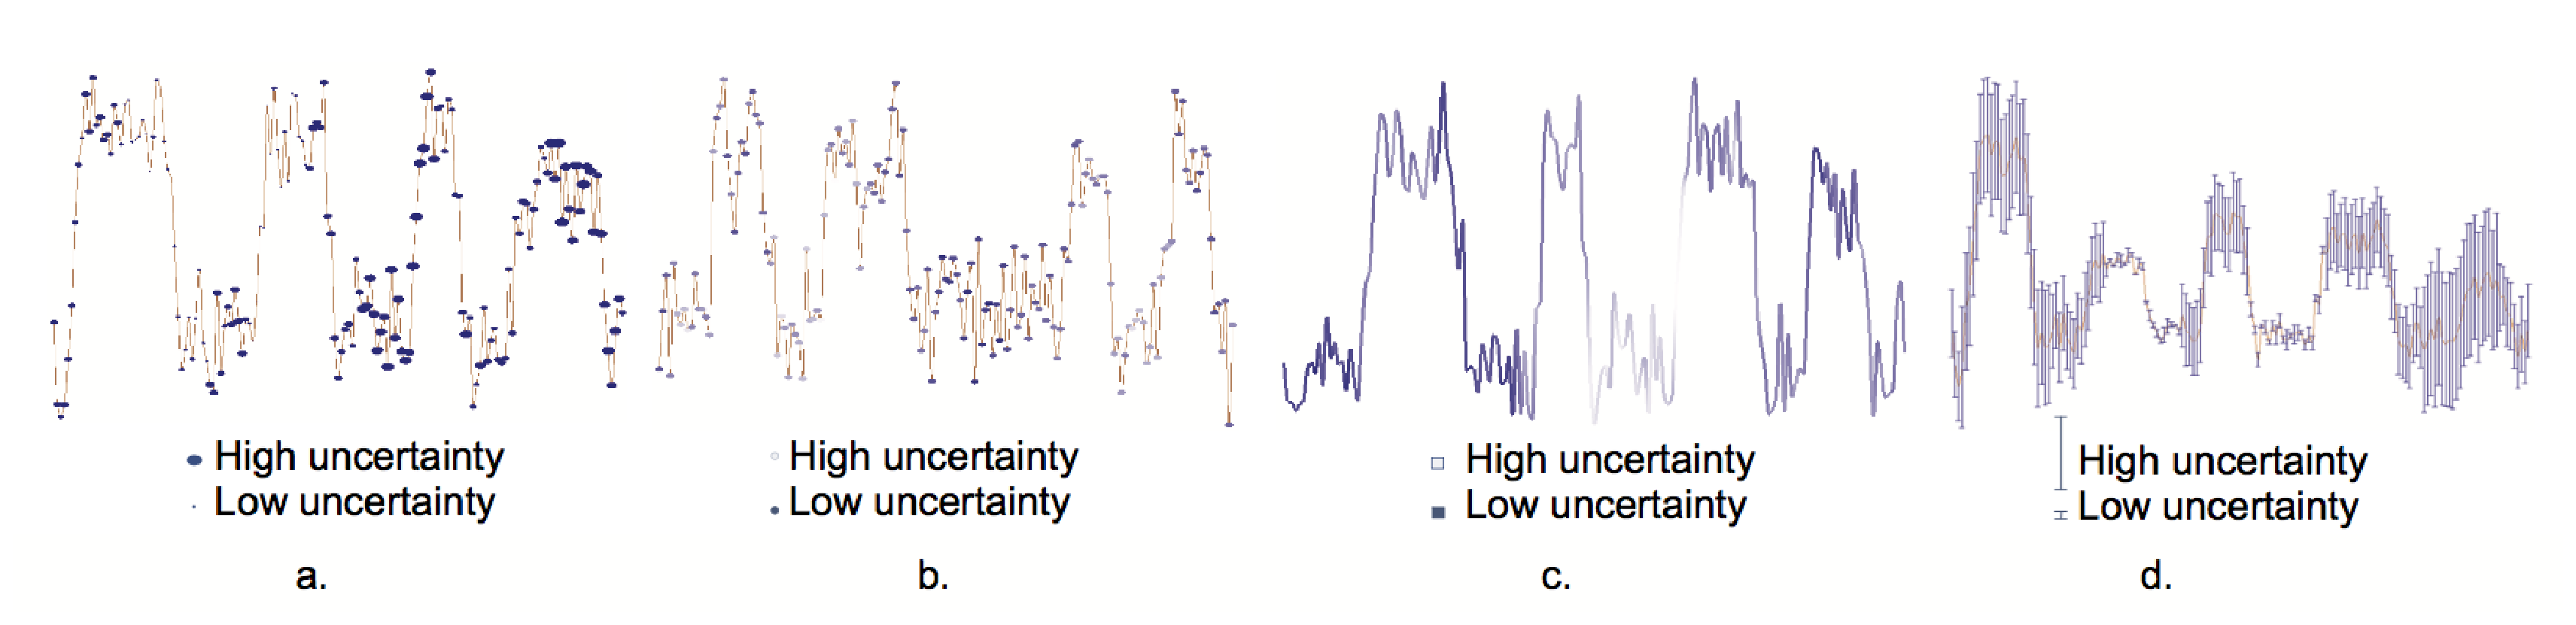
\includegraphics[width=1.0\columnwidth]{uncertainty}
	\caption{Uncertainty visualization techniques for exploring time series data. Image from Sanyal et al.~\cite{sanyal2009user}.}
	\label{fig:uncertainty}
\end{figure}

While aggregating customer data in a privacy-preserving manner is a strength of our proposed work, we observe that a tailored visualization is necessary to provide an intuitive analysis environment to our clients. 
A significant consideration in designing this visualization interface is the ability to communicate uncertainty associated with the aggregated data. 
In this portion of the project, we propose to explore techniques for visualizing uncertainty in time series data and demonstrate their usability.

Figure~\ref{fig:uncertainty} shows examples of existing designs for communicating data uncertainty.
Researchers have proposed several designs ~\cite{brodlie2012review,sanyal2009user,sanyal2010noodles,spiegelhalter2011visualizing} but few have been tested and usually with unrepresentative populations.  
To determine which technique is best for communicating uncertainty, we will rigorously examine existing methods. 
These include scaling the size of visual elements (Figure ~\ref{fig:uncertainty}a), using color to encode the degree of uncertainty (Figure ~\ref{fig:uncertainty}b), using transparency or blurring (Figure ~\ref{fig:uncertainty}c), and using standard error bars (Figure ~\ref{fig:uncertainty}d). 

%\paragraph{Exploring and evaluating techniques for communicating uncertainty to non-experts}
In this phase of the project, \emph{we will explore and evaluate methods for communicating uncertainty to non-experts}.
We plan first to test the designs using fictitious data with a diverse population of study participants via Amazon's Mechanical Turk. 
Once we have some candidate visualizations, we will expand these results by testing real aggregated data with clients in their natural work environments.
Dr. Ottley and her team have extensive experience in evaluating systems.
Here we outline the steps we will take to evaluate the different designs.   

\paragraph{Comparing Designs} 
Our goal here is to rank visualization designs based how effective they are at conveying meaningful information and facilitating decision-making.  
We will conduct experiments via Amazon's Mechanical Turk using three different evaluation approaches.
\begin{itemize}
\item[(1)] We will measure speed and accuracy as participants complete standard search and retrieval tasks.
\item[(2)] Participants will perform decision-making tasks, and we will investigate how each visualization impact the decisions made.
\item[(3)] During our experiment, we will conduct additional post-tests using adaptations of standard questionnaires. For instance, we will use the NASA-TLX for subjective measures of workload~\cite{hart1988development}, and the System Usability Scale for measuring perceived usability~\cite{bangor2008empirical}. 
\end{itemize}

\paragraph{Client Feedback}
Once we have narrowed the set of prospective visualizations, we will test these candidate designs with real clients. 
We will recruit participants from the BECS annual aquatic sales meeting.   
The clients will interact with the top designs from our previous rounds of experiments. 
For this set of user studies, we will conduct a qualitative evaluation by performing one-on-one observation and collecting clients' feedback.
A typical usability testing of this nature involves techniques such as “think-aloud” exercises, documentation of users’ reported insights, and the time they took to arrive at them~\cite{charlton2001handbook,hix1993developing,lewis1982using}. Findings from this round of testing will also be used to refine the visualization designs.

\paragraph{Application to Visualization Theory} 
Our proposed work of exploring techniques for communicating uncertainty has applications beyond our problem statement. Visualizing uncertainty is a central challenge in the Information Visualization community with many applications including weather, health, and government. Evaluating and potentially developing novel visualization techniques for representing uncertainty will be a signification contrition to these application areas.  


\subsubsection{Judging Success}

Ultimately, this project will be successful if we can effectively
protect the privacy of individual data contributors (i.e., a small
privacy budget) concurrently with releasing aggregate data that has
high utility (i.e., low uncertainty).  While theory tells us we cannot
be perfect at one without sacrificing the other, the intention
is to determine how close to that ultimate scenario it is to possible to be.

At the completion of Phase~I, a judgment is required to determine if
further effort towards the above ultimate goal is warranted.
Because that judgment is both a commercial and a technical judgment, we
plan to leverage BECS's annual aquatics sales meeting (which happens in
the fall, typically in November) to help us make that determination.

The sales meeting is timely, in that it happens towards the end of
the Phase~I schedule period.  It is also convenient, in that it is held
in St.~Louis and has attendees who are quite knowledgeable about 
the aquatics industry from around the country (and the world).
Finally, it is inexpensive (at least to the grant), because the full
costs of travel, meeting hall, etc., are all covered by BECS and
the attendees, no SBIR funds need be expended.

As described above, during the meeting we will solicit participants
to assist us in evaluating the most promising candidate data visualizations.
In addition, as part of the one-on-one assessment, we will seek their
input as to the levels of privacy that are acceptable and levels of 
uncertainty that are tolerable.
This is how we will judge whether or not we have been successful
in the Phase~I effort.

\subsection{Research Plan}
\label{sec:plan}

The primary participants in the project all reside in St. Louis, Missouri,
so face-to-face meetings have a relatively low overhead. We will coordinate
the project through periodic (e.g., biweekly) meetings that alternate
locations (one meeting at BECS Technology's facility, and two weeks later
another meeting on campus at Washington Univ. in St. Louis).

Dr. Fan is physically remote (she is in Albany, NY), so her primary
method of interaction will be via electronic communication.  We will
use video-conferencing fairly extensively when face-to-face discussions
are warranted.  In addition, the Dept.~of Computer Science and Engineering
at Washington University in St.~Louis
will invite Dr.~Fan to present a colloquium on campus at or very near
the beginning of the project.  This will enable all of the parties to
have a true face-to-face interaction without any travel expense charged
to the grant.

A formal agreement will need to be put in place between the company and
Washington~U.; however, the two organizations have collaborated in the
past (on a previous STTR grant through the National Institutes of Health).
The terms of that previous agreement will form the
basis of the required new agreement, and we anticipate no difficulties
in finalizing the agreement itself.

%\begin{figure}[h!]
%	\vspace{-0.2in}
%	\begin{ganttchart}[
%		x unit=0.8cm, 
%		y unit chart=0.45cm, 
%		y unit title=0.45cm, 
%		hgrid, 
%		vgrid,
%		bar/.append style={fill=black!20}]{1}{12}
%		\gantttitle{\footnotesize{Quarter 1}}{3}
%		\gantttitle{\footnotesize{Quarter 2}}{3}
%		\gantttitle{\footnotesize{Quarter 3}}{3}
%		\gantttitle{\footnotesize{Quarter 4}}{3} \\
%		%\gantttitle{\footnotesize{Phase 2}}{2} \\
%		\ganttbar{\footnotesize{R1: Aggregation?}}{1}{6} \ganttnewline
%		\ganttbar{\footnotesize{R1: Implementation? }}{1}{3}
%		\ganttbar{}{6}{12} \ganttnewline
%		\ganttbar{\footnotesize{R2: IRB application}}{1}{1} \ganttnewline
%		\ganttbar{\footnotesize{R2: Design and implementation}}{1}{4} \ganttnewline
%		\ganttbar{\footnotesize{R2: Testing and refinement}}{5}{10} \ganttnewline
%		\ganttbar{\footnotesize{R2: Data analysis}}{10}{12} \ganttnewline
%		\ganttbar{\footnotesize{System Integration}}{13}{14} \ganttnewline
%		\ganttbar{\footnotesize{System Evaluation}}{13}{14}
%	\end{ganttchart}
%	\vspace{-0.2in}
%\end{figure}

The proposed research is suited for a twelve-month research agenda.
The schedule is shown in Figure~\ref{fig:gantt}.
Both research components can be independently investigated,
primarily in parallel by the two organizations, coming together
in the assessments to be performed at the sales meeting.

\begin{figure}[h]
 \center
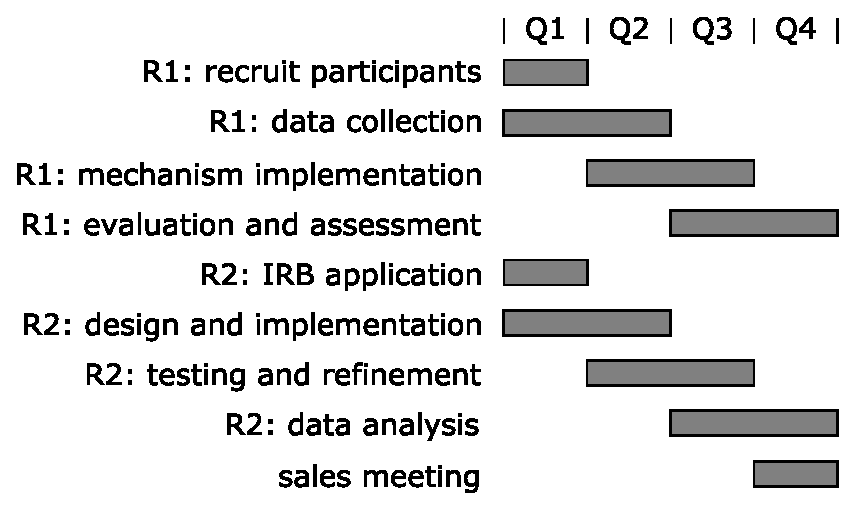
\includegraphics[width=0.6\columnwidth]{gantt}
    \caption{Project schedule, one year duration.}
    \label{fig:gantt}
\end{figure}

The results of the assessments during the sales meeting will inform
the activities to be pursued during Phase~II.
If the result of Phase~I is data that are appropriately anonymized,
one can consider the focus of Phase~II to be the determination of
what it is we can effectively learn from the anonymized data.

The learning from data will come in two forms:
\begin{itemize}
\item {\bf Machine learning} -- we will investigate utilizing techniques
described in the literature~\cite{acgmmtz16,fs10,ss15} for performing machine
learning on differentially private data sets.
We will apply techniques such as these to the problem of water treatment
control, with the goal of diminishing chemical consumption, providing
tighter control, and predicting issues that need human intervention
earlier than they can be detected presently.
\item {\bf Human learning} -- we will explore ways in which we can effectively
communicate to laypersons an intuitive notion of ``privacy budget,'' and
how to visualize risk, which has been studied in the
managment and
financial space~\cite{Eppler09,Sarlin16}, but we are unaware of any
work concerning privacy risk.
\end{itemize}

Also, during Phase~II we will investigate the applicability of techniques
we have learned about aquatics data to other domains.  This will start with
agriculture data, as we already have subscription-paying customers in
this market, so the business case could simply be made stronger, rather
than building it from the ground up.

\section{Broader Impacts}
\label{sec:broader}

Repeating a statement from Section~\ref{sec:opportunity},
we are interested in pursuing a scenario
where data owners are willing to share their data to enable some greater
good, with some reasable privacy assurances provided to those data owners.
This statement will be directly pursued in this project in the context of water
chemistry; however, it is a statement that is broadly applicable
across virtually all of the IoT space.
It's especially relevant to IoT in healthcare, where privacy concerns
are particularly acute.
BECS will seek to broaden it to BECS's other markets of agriculture
and refrigeration.
All of the data associated with NSF's Smart and Connected Communities
initiative has a similar set of privacy concerns.
In short, society can benefit to good answers to the questions we pose here.

At the graduate education level, this work will support two graduate
students at Washington Univ.~in St.~Louis.
The students will become versed in both visualization and
privacy theory, further strengthening their educational experience.

We will leverage a pair of existing university programs to help us
attract students from traditionally underrepresented groups.  The Olin
Fellowship Program (for women) and the Chancellor's Fellowship Program
(aimed at underrepresented minority students) have had a successful track
record of enabling individuals to pursue graduate study.  In our
experience, the most effective method for attracting students from
underrepresented groups is by personal contact with a suitable role
model.  To facilitate this, we regularly ask the appropriately
qualified individuals in our group to be actively involved in the
recruiting process.  This cohort currently includes both Dr.~Ottley
and one minority (African-American) student.

\section{Results of Prior SBIR/STTR Supported Research}
\label{sec:prior}

All information in this section
about other companies (Hearing Emulations, LLC, and
Exegy, Inc.), including quantities of both external and internal investments,
is proprietary to those firms.

\medskip

\noindent
{\bf Hearing Aids Based on Models of Cochlear Compression} --
SBIR Phase I (1999), \$100,000, and Phase II (2001), \$546,284.
PI: Julius Goldstein, Senior Personnel: Roger D. Chamberlain.

This research demonstrated improvements in the understandability of speech in
noisy environments for hearing-impaired individuals.
Commercialization of this work resulted in the formulation of a new
company, Hearing Emulations, LLC, which subsequently received private
investment of approximately \$2 million.
BECS's interest was sold to the investors, so we no longer
have visibility into the company.
Publications resulting from this work
include~\cite{ccd+02a,ccd+02b,chmw03,cgi03,Gold06,gogv03b,gogv03,gvc01,gvcgi00}.
Patents resulting from this work
include~\cite{Goldstein05a,Goldstein05b,gc03}.

\medskip

\noindent
{\bf Fast Biosequence Annotation via Reconfigurable Hardware} --
STTR Phase I (2004), \$307,508, and Phase II (2007), \$510,614.
PI: Jeremy Buhler, Senior Personnel: Roger D. Chamberlain.

This research resulted in FPGA-based accelerated implementations of
several biosequence applications, including both DNA and protein alignment
as well as RNA folding.
Commercialization of this work resulted in a Memorandum of Understanding (MOU)
between Exegy, Inc., and BECS.  Exegy has subsequently invested
approximately \$500,000 in the technology.
Under the terms of the MOU, Exegy
is not required to disclose sales figures to BECS.
Publications resulting from this work
include~\cite{bljc07,dlmbc10,hjlbc07,jbc08,jlbc07b,jlbc07a,jlbhc08,jbc09,jbc10b,jbc10a,kbcfgl04,kbcfgjl07,lbc05,lbc09},
which includes a best paper award~\cite{jbc10b}.
Patents resulting from this work
include~\cite{Buhler11,Buhler13,Buhler17} and one pending application.

\section{Conclusion}
\label{sec:conclude}

It is clear that privacy of IoT-derived data is currently a challenge,
and differential privacy theory has the potential to put privacy practice
on a sound theoretical footing.  What still remains to be seen is whether
or not differential privacy theory is ``ready for prime time.''

Specifically, can the current state of the theory handle all of the
practical considerations that much be resolved for it to be effective
in the real world.
\begin{itemize}
\item Can we choose appropriate parameter values so as to achieve
sufficient privacy and maintain data utility?
\item Can we effectively communicate the anonymized query results to
users in visual forms that include the inherent uncertainty due to privacy?
\item Can we combine differential privacy theory with other privacy
mechanisms for a multi-tiered privacy infrastructure?
\item While ensuring that cross-organizational data are private, can we
exploit those data to improve the practice of water treatment control?
\end{itemize}
These are the questions we intend to address as part of this SBIR project.
Success will enable benefits across many more markets than just aquatics,
as virtually all of the IoT space has issues that, if not identical to
those we face, are certainly comparable.


\clearpage
% \begin{scriptsize}
\bibliographystyle{abbrv}
\bibliography{prop}
% \end{scriptsize}

\end{document}

ize}

\end{document}

